\documentclass{beamer}
\usepackage[utf8]{inputenc}
\usepackage{graphicx, epsfig}
\usepackage{amsmath,mathrsfs,amsfonts,amssymb}
\usepackage{floatflt}
\usepackage{epic,ecltree}
\usepackage{mathtext}
\usepackage{fancybox}
\usepackage{fancyhdr}
\usepackage{multirow}
\usepackage{enumerate}
\usepackage{epstopdf}
\usepackage{multicol}
\usepackage{algorithm}
\usepackage[noend]{algorithmic}
\usepackage{tikz}
\usepackage{blindtext}
\usetheme{default}%{Singapore}%{Warsaw}%{Warsaw}%{Darmstadt}
\usecolortheme{default}

\setbeamerfont{title}{size=\Huge}
\setbeamertemplate{footline}[page number]{}

\setbeamertemplate{section in toc}[sections numbered]


\makeatletter
\newcommand\HUGE{\@setfontsize\Huge{35}{40}}
\makeatother    

\setbeamerfont{title}{size=\HUGE}
\beamertemplatenavigationsymbolsempty

% latin bold lower
\newcommand{\ba}{\mathbf{a}} 
\newcommand{\bc}{\mathbf{c}} 
\newcommand{\be}{\mathbf{e}} 
\newcommand{\bh}{\mathbf{h}} 
\newcommand{\bp}{\mathbf{p}} 
\newcommand{\bt}{\mathbf{t}} 
\newcommand{\bs}{\mathbf{s}} 
\newcommand{\bu}{\mathbf{u}} 
\newcommand{\bv}{\mathbf{v}} 
\newcommand{\bw}{\mathbf{w}} 
\newcommand{\bx}{\mathbf{x}} 
\newcommand{\by}{\mathbf{y}} 
\newcommand{\bz}{\mathbf{z}} 

% latin bold upper
\newcommand{\bA}{\mathbf{A}} 
\newcommand{\bB}{\mathbf{B}} 
\newcommand{\bC}{\mathbf{C}} 
\newcommand{\bI}{\mathbf{I}} 
\newcommand{\bJ}{\mathbf{J}} 
\newcommand{\bL}{\mathbf{L}} 
\newcommand{\bM}{\mathbf{M}} 
\newcommand{\bP}{\mathbf{P}}
\newcommand{\bQ}{\mathbf{Q}} 
\newcommand{\bR}{\mathbf{R}} 
\newcommand{\bT}{\mathbf{T}} 
\newcommand{\bU}{\mathbf{U}} 
\newcommand{\bV}{\mathbf{V}} 
\newcommand{\bW}{\mathbf{W}} 
\newcommand{\bX}{\mathbf{X}} 
\newcommand{\bY}{\mathbf{Y}} 
\newcommand{\bZ}{\mathbf{Z}} 

% latin cal upper
\newcommand{\cF}{\mathcal{F}} 
\newcommand{\cG}{\mathcal{G}} 
\newcommand{\cI}{\mathcal{I}} 
\newcommand{\cL}{\mathcal{L}} 
\newcommand{\cM}{\mathcal{M}} 
\newcommand{\cN}{\mathcal{N}} 
\newcommand{\cS}{\mathcal{S}} 
\newcommand{\cT}{\mathcal{T}} 
\newcommand{\cW}{\mathcal{W}} 
\newcommand{\cX}{\mathcal{X}} 
\newcommand{\cZ}{\mathcal{Z}} 

% latin bb upper
\newcommand{\bbE}{\mathbb{E}} 
\newcommand{\bbI}{\mathbb{I}} 
\newcommand{\bbP}{\mathbb{P}} 
\newcommand{\bbR}{\mathbb{R}} 

% greek bold lower
\newcommand{\bepsilon}{\boldsymbol{\epsilon}} 
\newcommand{\btheta}{\boldsymbol{\theta}} 
\newcommand{\blambda}{\boldsymbol{\lambda}} 
\newcommand{\bpi}{\boldsymbol{\pi}} 
\newcommand{\bmu}{\boldsymbol{\mu}} 
\newcommand{\bsigma}{\boldsymbol{\sigma}} 
\newcommand{\bphi}{\boldsymbol{\phi}} 

% greek bold upper
\newcommand{\bSigma}{\boldsymbol{\Sigma}} 

\DeclareMathOperator*{\argmin}{arg\,min}
\DeclareMathOperator*{\argmax}{arg\,max}

\newcommand{\createdgmtitle}[1]{\title[\hbox to 56mm{Deep Generative Models  \hfill\insertframenumber\,/\,\inserttotalframenumber}]
	{Deep Generative Models \\ {\Huge Lecture #1}}
	\author{Roman Isachenko}
	\institute{
\includegraphics[width=0.5cm]{../utils/ozonmasterslogo} \large{Ozon Masters}}
	\date{Spring, 2022}
}

\usepackage{tikz}
\usetikzlibrary{arrows,shapes,positioning,shadows,trees}

\newcommand\myfootnote[1]{%
  \tikz[remember picture,overlay]
  \draw (current page.south west) +(1in + \oddsidemargin,0.5em)
  node[anchor=south west,inner sep=0pt]{\parbox{\textwidth}{%
      \rlap{\rule{10em}{0.4pt}}\raggedright\scriptsize \textit{#1}}};}

\newcommand\myfootnotewithlink[2]{%
  \tikz[remember picture,overlay]
  \draw (current page.south west) +(1in + \oddsidemargin,0.5em)
  node[anchor=south west,inner sep=0pt]{\parbox{\textwidth}{%
      \rlap{\rule{10em}{0.4pt}}\raggedright\scriptsize\href{#1}{\textit{#2}}}};}
      
\AtBeginSection[]
{
	\begin{frame}{Outline}
		\tableofcontents[currentsection,subsectionstyle=hide]
	\end{frame}
}
\AtBeginSubsection[]{
	\begin{frame}{Outline}
		\tableofcontents[currentsection,currentsubsection]
	\end{frame}
}
\createdgmtitle{6}
%--------------------------------------------------------------------------------
\begin{document}
%--------------------------------------------------------------------------------
\begin{frame}[noframenumbering,plain]
%\thispagestyle{empty}
\titlepage
\end{frame}
%=======
\begin{frame}{Recap of previous lecture}
	\begin{block}{MLE problem}
		\vspace{-0.3cm}
		\[
		p(\bx|\btheta) = p(\bz) \left|\det \left(  \frac{\partial \bz}{\partial \bx} \right) \right|  = p(f(\bx, \btheta)) \left|\det \left( \frac{\partial f(\bx, \btheta)}{\partial \bx} \right) \right|
		\]
		\[
		\log p(\bx|\btheta) = \log p(f(\bx, \btheta)) + \log  |\det (\bJ_f) | \rightarrow \max_{\btheta}
		\]
	\end{block}
	\vspace{-0.2cm}
	\begin{figure}
		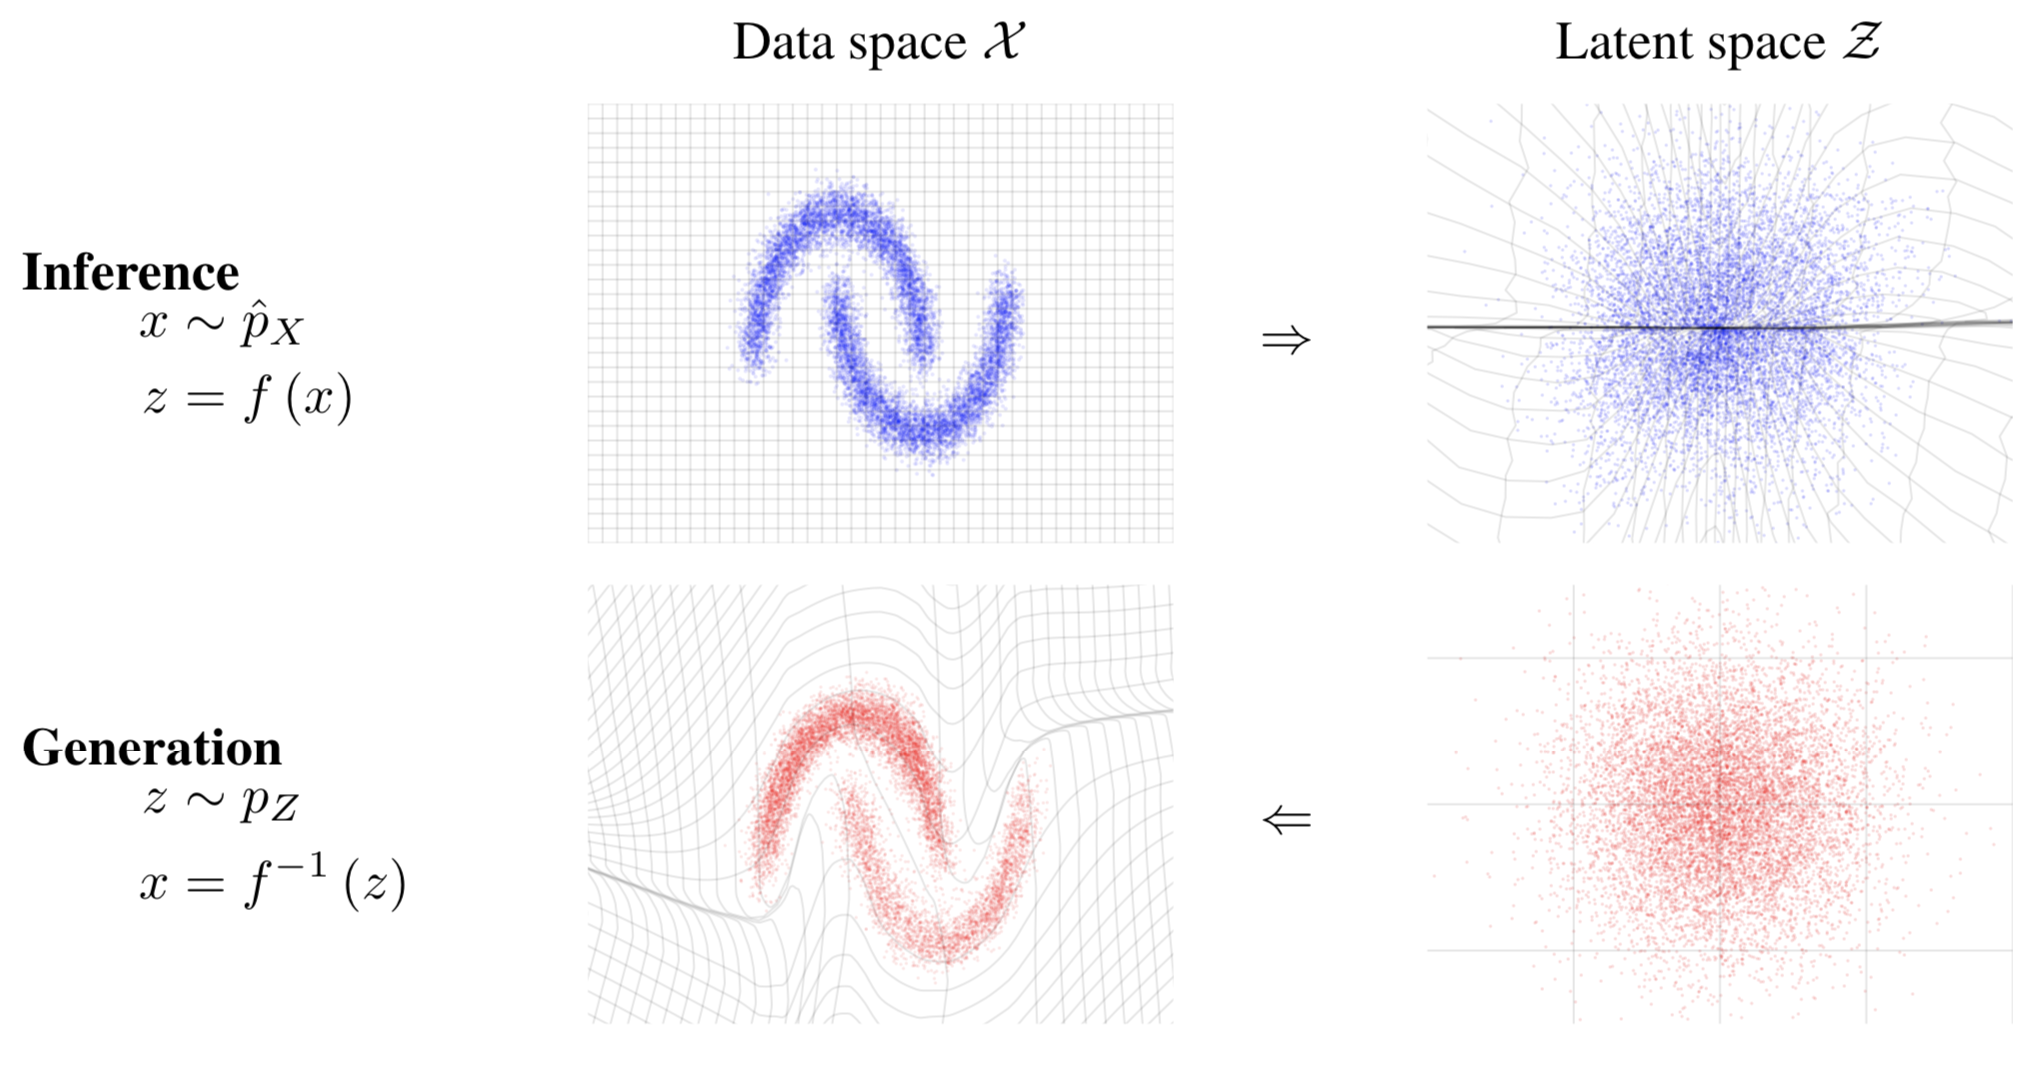
\includegraphics[width=0.85\linewidth]{figs/flows_how2}
	\end{figure}
	\myfootnotewithlink{https://arxiv.org/abs/1605.08803}{Dinh L., Sohl-Dickstein J., Bengio S. Density estimation using Real NVP, 2016} 
\end{frame}
%=======
\begin{frame}{Recap of previous lecture}
	\[
		\log p(\bx|\btheta) = \log p(f(\bx, \btheta)) + \log  |\det (\bJ_f) | \rightarrow \max_{\btheta}
	\]
	\vspace{-0.3cm}
	\begin{block}{Definition}
		Normalizing flow is a \textit{differentiable, invertible} mapping from data $\bx$ to the noise $\bz$. 
	\end{block}
	\begin{itemize}
		\item \textbf{Normalizing} means that the inverse flow takes samples from $p(\bx)$ and normalizes them into samples from density $p(\bz)$.
		\item \textbf{Flow} refers to the trajectory followed by samples from $p(\bz)$ as they are transformed by the sequence of transformations
		\[
			\bz = f_K \circ \dots \circ f_1(\bx); \quad \bx = f_1^{-1} \circ \dots \circ f_K^{-1} (\bz) = g_1 \circ \dots \circ g_K(\bz) 
		\] 
		\vspace{-0.4cm}
		\begin{block}{Log likelihood}
			\vspace{-0.4cm}
			\[
				\log p(\bx | \btheta) = \log p(f_K \circ \dots \circ f_1(\bx)) + \sum_{k=1}^K\log |\det (\bJ_{f_k})|,
			\]
			\vspace{-0.4cm} \\
			where $\bJ_{f_k} = \frac{\partial \mathbf{f}_k}{\partial \mathbf{f}_{k-1}}$.
		\end{block}
	\end{itemize}
\end{frame}
%=======
\begin{frame}{Recap of previous lecture}
	\begin{block}{Forward KL for flow model}
	  	\vspace{-0.1cm}
		\[
			\log p(\bx|\btheta) = \log p(f(\bx, \btheta)) + \log  |\det (\bJ_f)|
		\]
		\vspace{-0.3cm}
	\end{block}
	\begin{block}{Reverse KL for flow model}
  		\vspace{-0.5cm}
		\[
			KL(p || \pi)  = \bbE_{p(\bz)} \left[  \log p(\bz) -  \log |\det (\bJ_g)| - \log \pi(g(\bz, \btheta)) \right]
		\]
		\vspace{-0.5cm}
	\end{block}
	\begin{block}{Flow KL duality}
	  	\vspace{-0.3cm}
		\[
			\argmin_{\btheta} KL(\pi(\bx) || p(\bx | \btheta)) = \argmin_{\btheta} KL(p(\bz | \btheta) || p(\bz)).
		\]
		\vspace{-0.3cm}
		\begin{itemize}
			\item $p(\bz)$ is a base distribution; $\pi(\bx)$ is a data distribution;
			\item $\bz \sim p(\bz)$, $\bx = g(\bz, \btheta)$, $\bx \sim p(\bx| \btheta)$;
			\item $\bx \sim \pi(\bx)$, $\bz = f(\bx, \btheta)$, $\bz \sim p(\bz | \btheta)$;
		\end{itemize}
	\end{block}
	\myfootnotewithlink{https://arxiv.org/abs/1912.02762}{Papamakarios G. et al. Normalizing flows for probabilistic modeling and inference, 2019} 
\end{frame}
%=======
\begin{frame}{Recap of previous lecture}
	\vspace{-0.5cm}
	\begin{block}{Flow log-likelihood}
		\vspace{-0.3cm}
		\[
			\log p(\bx|\btheta) = \log p(f(\bx, \btheta)) + \log  |\det (\bJ_f)|
		\]
		\vspace{-0.5cm}
	\end{block}
	The main challenge is a determinant of the Jacobian.
	\begin{block}{Residual flows: planar/Sylvester}
		\vspace{-0.7cm}
		\[
			g(\bz, \btheta) = \bz + \mathbf{u} \, \sigma(\bw^T\bz + b); \quad 
			g(\bz, \btheta) = \bz + \bA \, \sigma(\bB\bz + \mathbf{b}).
		\]
		Matrix determinant lemma for calculating the Jacobian.
	\end{block}
	\begin{block}{Linear flows}	
		\vspace{-0.2cm}
		\[
			\bz = f(\bx, \btheta) = \bW \bx, \quad \bW \in \bbR^{m \times m}, \quad \btheta = \bW, \quad \bJ_f = \bW
		\]
		Matrix decompositions (LU or QR helps to parametrize matrix $\bW$ and reduce the cost of computing the $det(\bJ)$).
	\end{block}
	\myfootnote{\href{https://arxiv.org/abs/1505.05770}{Rezende D. J., Mohamed S. Variational Inference with Normalizing Flows, 2015}\\
	\href{https://arxiv.org/abs/1803.05649}{Berg R. et al. Sylvester normalizing flows for variational inference, 2018} \\
	\href{https://arxiv.org/abs/1807.03039}{Kingma D. P., Dhariwal P. Glow: Generative Flow with Invertible 1x1 Convolutions, 2018}}
\end{frame}
%=======
\begin{frame}{Outline}
	\tableofcontents
\end{frame}
%=======
\begin{frame}{Autoregressive flows}
	\vspace{-0.3cm}
	\[
	x_j = \tau (z_j, c(\bz_{1:j-1})) \quad \Leftrightarrow \quad z_j = \tau^{-1} (x_j, c(\bz_{1:j-1}))
	\]
	\vspace{-0.3cm}
	\begin{itemize}
		\item $\tau (\cdot, \cdot)$ -- coupling law (invertible by first argument, differentiable).
		\item $c(\cdot)$ -- coupling function (do not need to be invertible, could be neural network).
	\end{itemize}
	\begin{block}{Coupling law $\tau(\cdot, \cdot)$}
		\begin{itemize}
			\item $\tau(x, c) = x + c$ -- additive;
			\item $\tau(x, c) = x \odot c_1 + c_2$ -- affine.
		\end{itemize}
	\end{block}
	What is the Jacobian for the additive/affine coupling law? 
	\begin{block}{Jacobian}
		\vspace{-0.3cm}
		\[
		\det \left( \frac{\partial \bx}{\partial \bz} \right) = \prod_{j=1}^m \frac{\partial x_j}{\partial z_j} = \prod_{j=1}^m \frac{\partial \tau (z_j, c(\bz_{1:j-1})) }{\partial z_j}
		\]
		\vspace{-0.3cm}
	\end{block}
	
	\myfootnotewithlink{https://arxiv.org/abs/1912.02762}{Papamakarios G. et al. Normalizing flows for probabilistic modeling and inference, 2019} 
\end{frame}
%=======
\begin{frame}{Autoregressive flows}
	\begin{block}{Forward and inverse transforms}
		\[
		x_j = \tau (z_j, c(\bz_{1:j-1})) \quad \Leftrightarrow \quad z_j = \tau^{-1} (x_j, c(\bz_{1:j-1}))
		\]
		\begin{figure}
			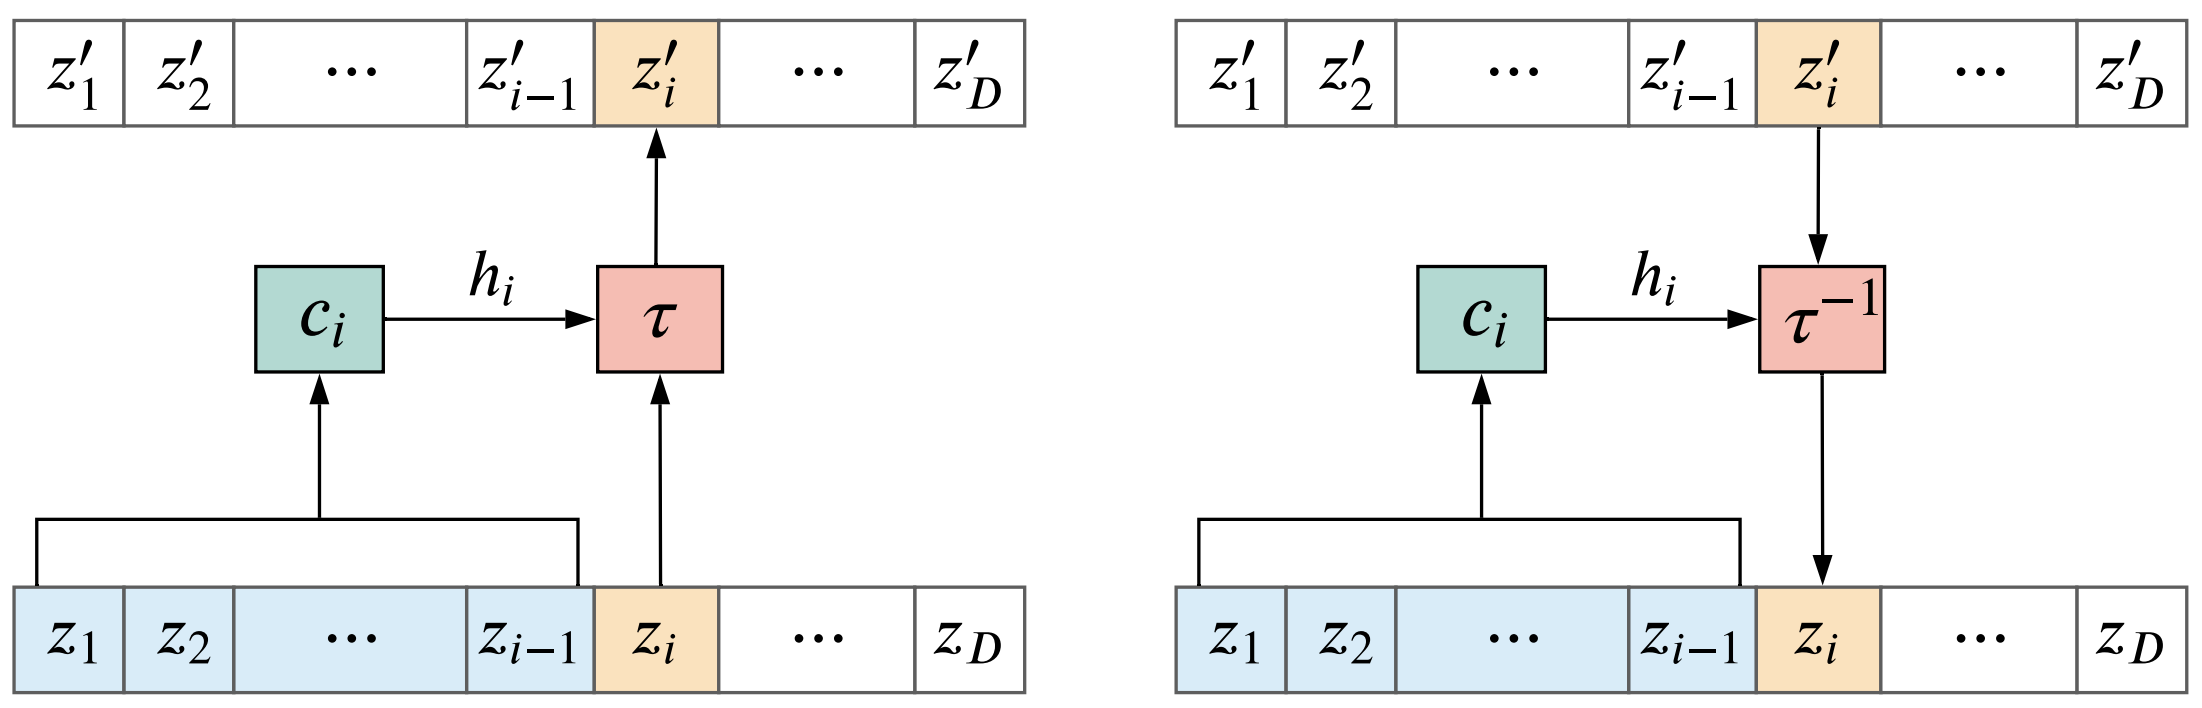
\includegraphics[width=\linewidth]{figs/autoregressive_flow}
		\end{figure}
	\end{block}
	\begin{itemize}
		\item Forward transform is \textbf{not sequential}.
		\item Inverse transform is \textbf{sequential}.
	\end{itemize}
	
	\myfootnotewithlink{https://arxiv.org/abs/1912.02762}{Papamakarios G. et al. Normalizing flows for probabilistic modeling and inference, 2019} 
\end{frame}
%=======
\section{RealNVP: coupling layer}
%=======
\begin{frame}{RealNVP}
	\begin{block}{Coupling layer}
		\vspace{-0.8cm}
		\begin{equation*}
			\begin{cases} \bz_{1:d} = \bx_{1:d}; \\ \bz_{d:m} = \tau (\bx_{d:m}, c(\bx_{1:d}));\end{cases} 
			\quad \Leftrightarrow \quad 
			\begin{cases} \bx_{1:d} = \bz_{1:d}; \\ \bx_{d:m} = \tau^{-1} (\bz_{d:m}, c(\bz_{1:d})).\end{cases}
		\end{equation*}
		\vspace{-0.5cm}
	\end{block}
	\begin{block}{Image partitioning}
		\begin{figure}
			\centering
			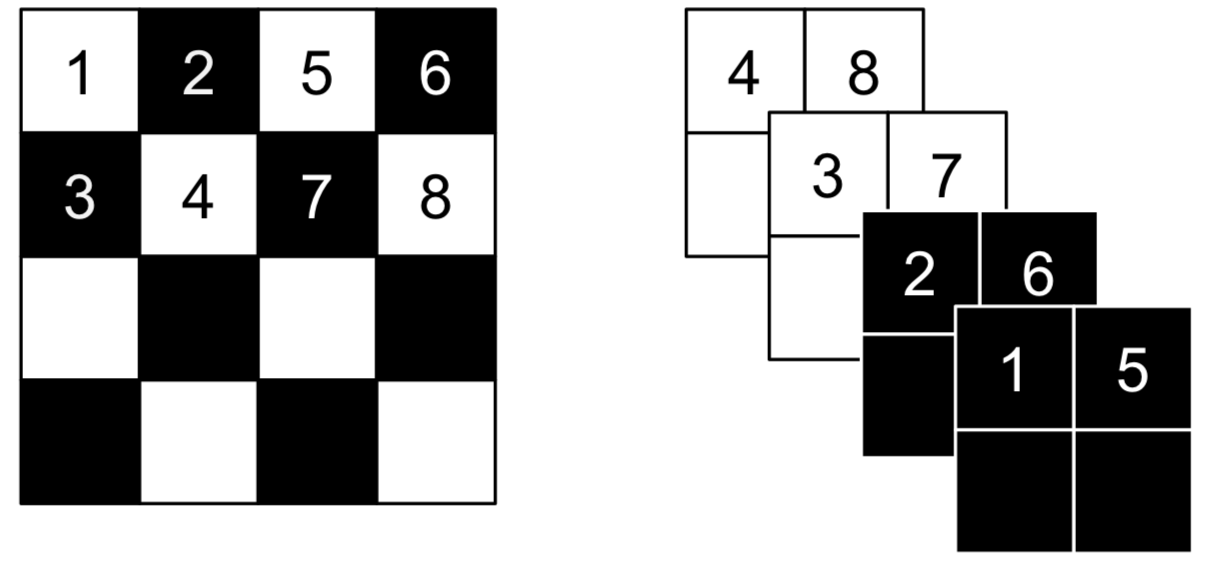
\includegraphics[width=0.65\linewidth]{figs/realnvp_masking.png}
		\end{figure}
	\end{block}
	\vspace{-0.5cm}
	
	Checkerboard ordering uses masking, channelwise ordering uses splitting.
	\myfootnotewithlink{https://arxiv.org/abs/1410.8516}{Dinh L., Krueger D., Bengio Y. NICE: Non-linear Independent Components Estimation, 2014}
\end{frame}
%=======
\begin{frame}{RealNVP}
	\begin{block}{Affine coupling law}
		\[
			\begin{cases} \bz_{1:d} = \bx_{1:d}; \\ \bz_{d:m} = \bx_{d:m} \odot c_1(\bx_{1:d}, \btheta) + c_2(\bx_{1:d}, \btheta).\end{cases} 
		\]
		\[
			\begin{cases} \bx_{1:d} = \bz_{1:d}; \\ \bx_{d:m} = \left(\bz_{d:m} - c_2(\bz_{1:d}, \btheta) \right) \cdot \frac{1}{c_1(\bz_{1:d}, \btheta)}.\end{cases}
		\]
	\end{block}
	\begin{block}{Jacobian}
		\vspace{-0.5cm}
		\[
		\det \left( \frac{\partial \bz}{\partial \bx} \right) = \det 
		\begin{pmatrix}
			\bI_d & 0_{d \times m - d} \\
			\frac{\partial \bz_{d:m}}{\partial \bx_{1:d}} & \frac{\partial \bz_{d:m}}{\partial \bx_{d:m}}
		\end{pmatrix} = \prod_{j=1}^{m - d} c_1(\bx_{1:d}, \btheta)_j.
		\]
		Non-Volume Preserving (the determinant of Jacobian $\neq 1$).
	\end{block}
	
	\myfootnotewithlink{https://arxiv.org/abs/1605.08803}{Dinh L., Sohl-Dickstein J., Bengio S. Density estimation using Real NVP, 2016} 
\end{frame}
%=======
\begin{frame}{AF vs IAF vs RealNVP}
	\begin{block}{MADE/AF}
		\vspace{-0.5cm}
		\[
		\bx = \bsigma (\bx) \odot \bz + \bmu(\bx).
		\]
		Estimating the density $p(\bx | \btheta)$ - 1 pass, sampling - $m$ passes.
	\end{block}
	\begin{block}{IAF}
		\vspace{-0.5cm}
		\[
		\bx = \tilde{\bsigma} (\bz) \odot \bz + \tilde{\bmu}(\bz).
		\]
		Estimating the density $p(\bx | \btheta)$ - $m$ passes, sampling - 1 pass.
	\end{block}
	\begin{block}{RealNVP}
		\vspace{-0.2cm}
		\[
			\begin{cases}
				\bx_{1:d} &= \bz_{1:d}; \\ 
				\bx_{d:m} &= \bz_{d:m} \odot c_1(\bz_{1:d}, \btheta) + c_2(\bz_{1:d}, \btheta).
			\end{cases}
		\]
		\vspace{-0.5cm}
		Estimating the density $p(\bx | \btheta)$ - 1 pass, sampling - 1 pass.
	\end{block}
	\myfootnotewithlink{https://arxiv.org/abs/1705.07057}{Papamakarios G., Pavlakou T., Murray I. Masked Autoregressive Flow for Density Estimation, 2017} 
\end{frame}
%=======
\begin{frame}{AF vs IAF vs RealNVP}
	\begin{block}{RealNVP}
		\vspace{-0.3cm}
		\[
			\begin{cases}
				\bx_{1:d} &= \bz_{1:d}; \\ 
				\bx_{d:m} &= \bz_{d:m} \odot c_1(\bz_{1:d}, \btheta) + c_2(\bz_{1:d}, \btheta).
			\end{cases}
		\]
		\vspace{-0.3cm}
	\end{block}
	\begin{itemize}
		\item Calculating the density $p(\bx | \btheta)$ - 1 pass.
		\item Sampling - 1 pass.
	\end{itemize}
	
	RealNVP is a special case of AF and IAF:
	\begin{block}{AF}
		\vspace{-0.5cm}
		\begin{equation*}
			\begin{cases}
				\mu_j  = 0, \sigma_j = 1, \, j = 1, \dots, d; \\
				\mu_j, \sigma_j \text{ -- functions of } \bx_{1:d}, \, j = d+1, \dots, m.
			\end{cases}
		\end{equation*}
		\vspace{-0.3cm}
	\end{block}
	\begin{block}{IAF}
		\vspace{-0.3cm}
		\begin{equation*}
			\begin{cases}
				\tilde{\mu}_j = 0, \tilde{\sigma}_j = 1, \, j = 1, \dots, d; \\
				\tilde{\mu}_j, \tilde{\sigma}_j \text{ -- functions of } \bz_{1:d}, \, j = d+1, \dots, m.
			\end{cases}
		\end{equation*}
	\end{block}
	\myfootnotewithlink{https://arxiv.org/abs/1705.07057}{Papamakarios G., Pavlakou T., Murray I. Masked Autoregressive Flow for Density Estimation, 2017} 
\end{frame}
%=======
\begin{frame}{RealNVP samples}
		\begin{figure}
			\centering
			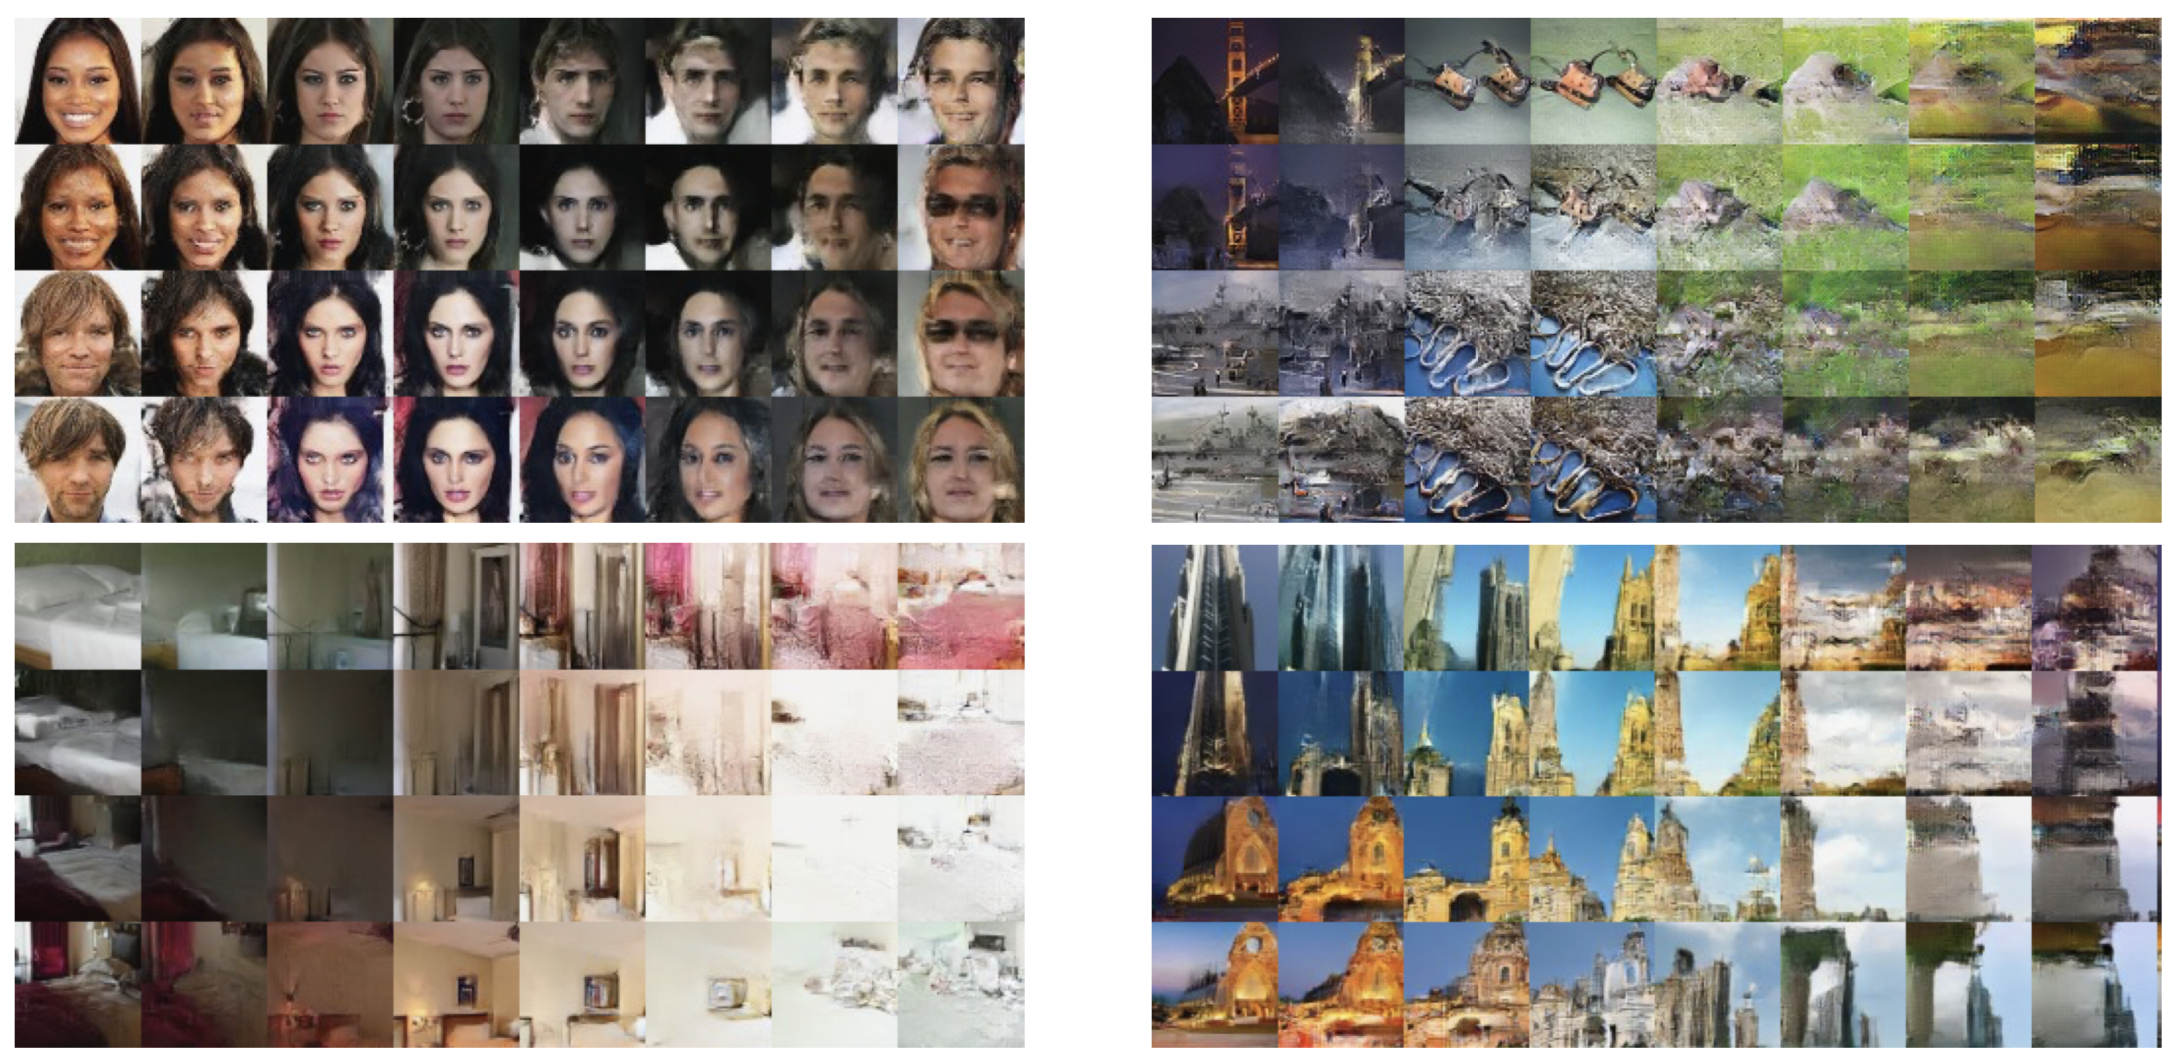
\includegraphics[width=\linewidth]{figs/realnvp_output.png}
		\end{figure}
	\myfootnotewithlink{https://arxiv.org/abs/1605.08803}{Dinh L., Sohl-Dickstein J., Bengio S. Density estimation using Real NVP, 2016} 
\end{frame}
%=======
\begin{frame}{Linear flows}
	\begin{block}{RealNVP}
		\vspace{-0.5cm}
		\begin{equation*}
			\begin{cases} \bz_{1:d} = \bx_{1:d}; \\ \bz_{d:m} = \tau (\bx_{d:m}, c(\bx_{1:d}));\end{cases} 
			\quad \Leftrightarrow \quad 
			\begin{cases} \bx_{1:d} = \bz_{1:d}; \\ \bx_{d:m} = \tau^{-1} (\bz_{d:m}, c(\bz_{1:d})).\end{cases}
		\end{equation*}
		\vspace{-0.2cm}
	\end{block}
	\begin{itemize}
	\item First step is a \textbf{split} operator which decouples a variable into 2 subparts: $\bx_1$ and $\bx_2$ (usualy channel-wise).
	\item We should \textbf{permute} components between different layers.
	\end{itemize}
	\[
		\bz = \bW \bx, \quad \bW \in \bbR^{m \times m}
	\]
	In general, we need $O(m^3)$ to invert matrix.
	\begin{block}{Invertibility}
		\begin{itemize}
			\item Diagonal matrix $O(m)$.
			\item Triangular matrix $O(m^2)$.
			\item It is impossible to parametrize all invertible matrices.
		\end{itemize}
	\end{block}
\end{frame}
%=======
\begin{frame}{Glow samples}
	\begin{figure}
		\centering
		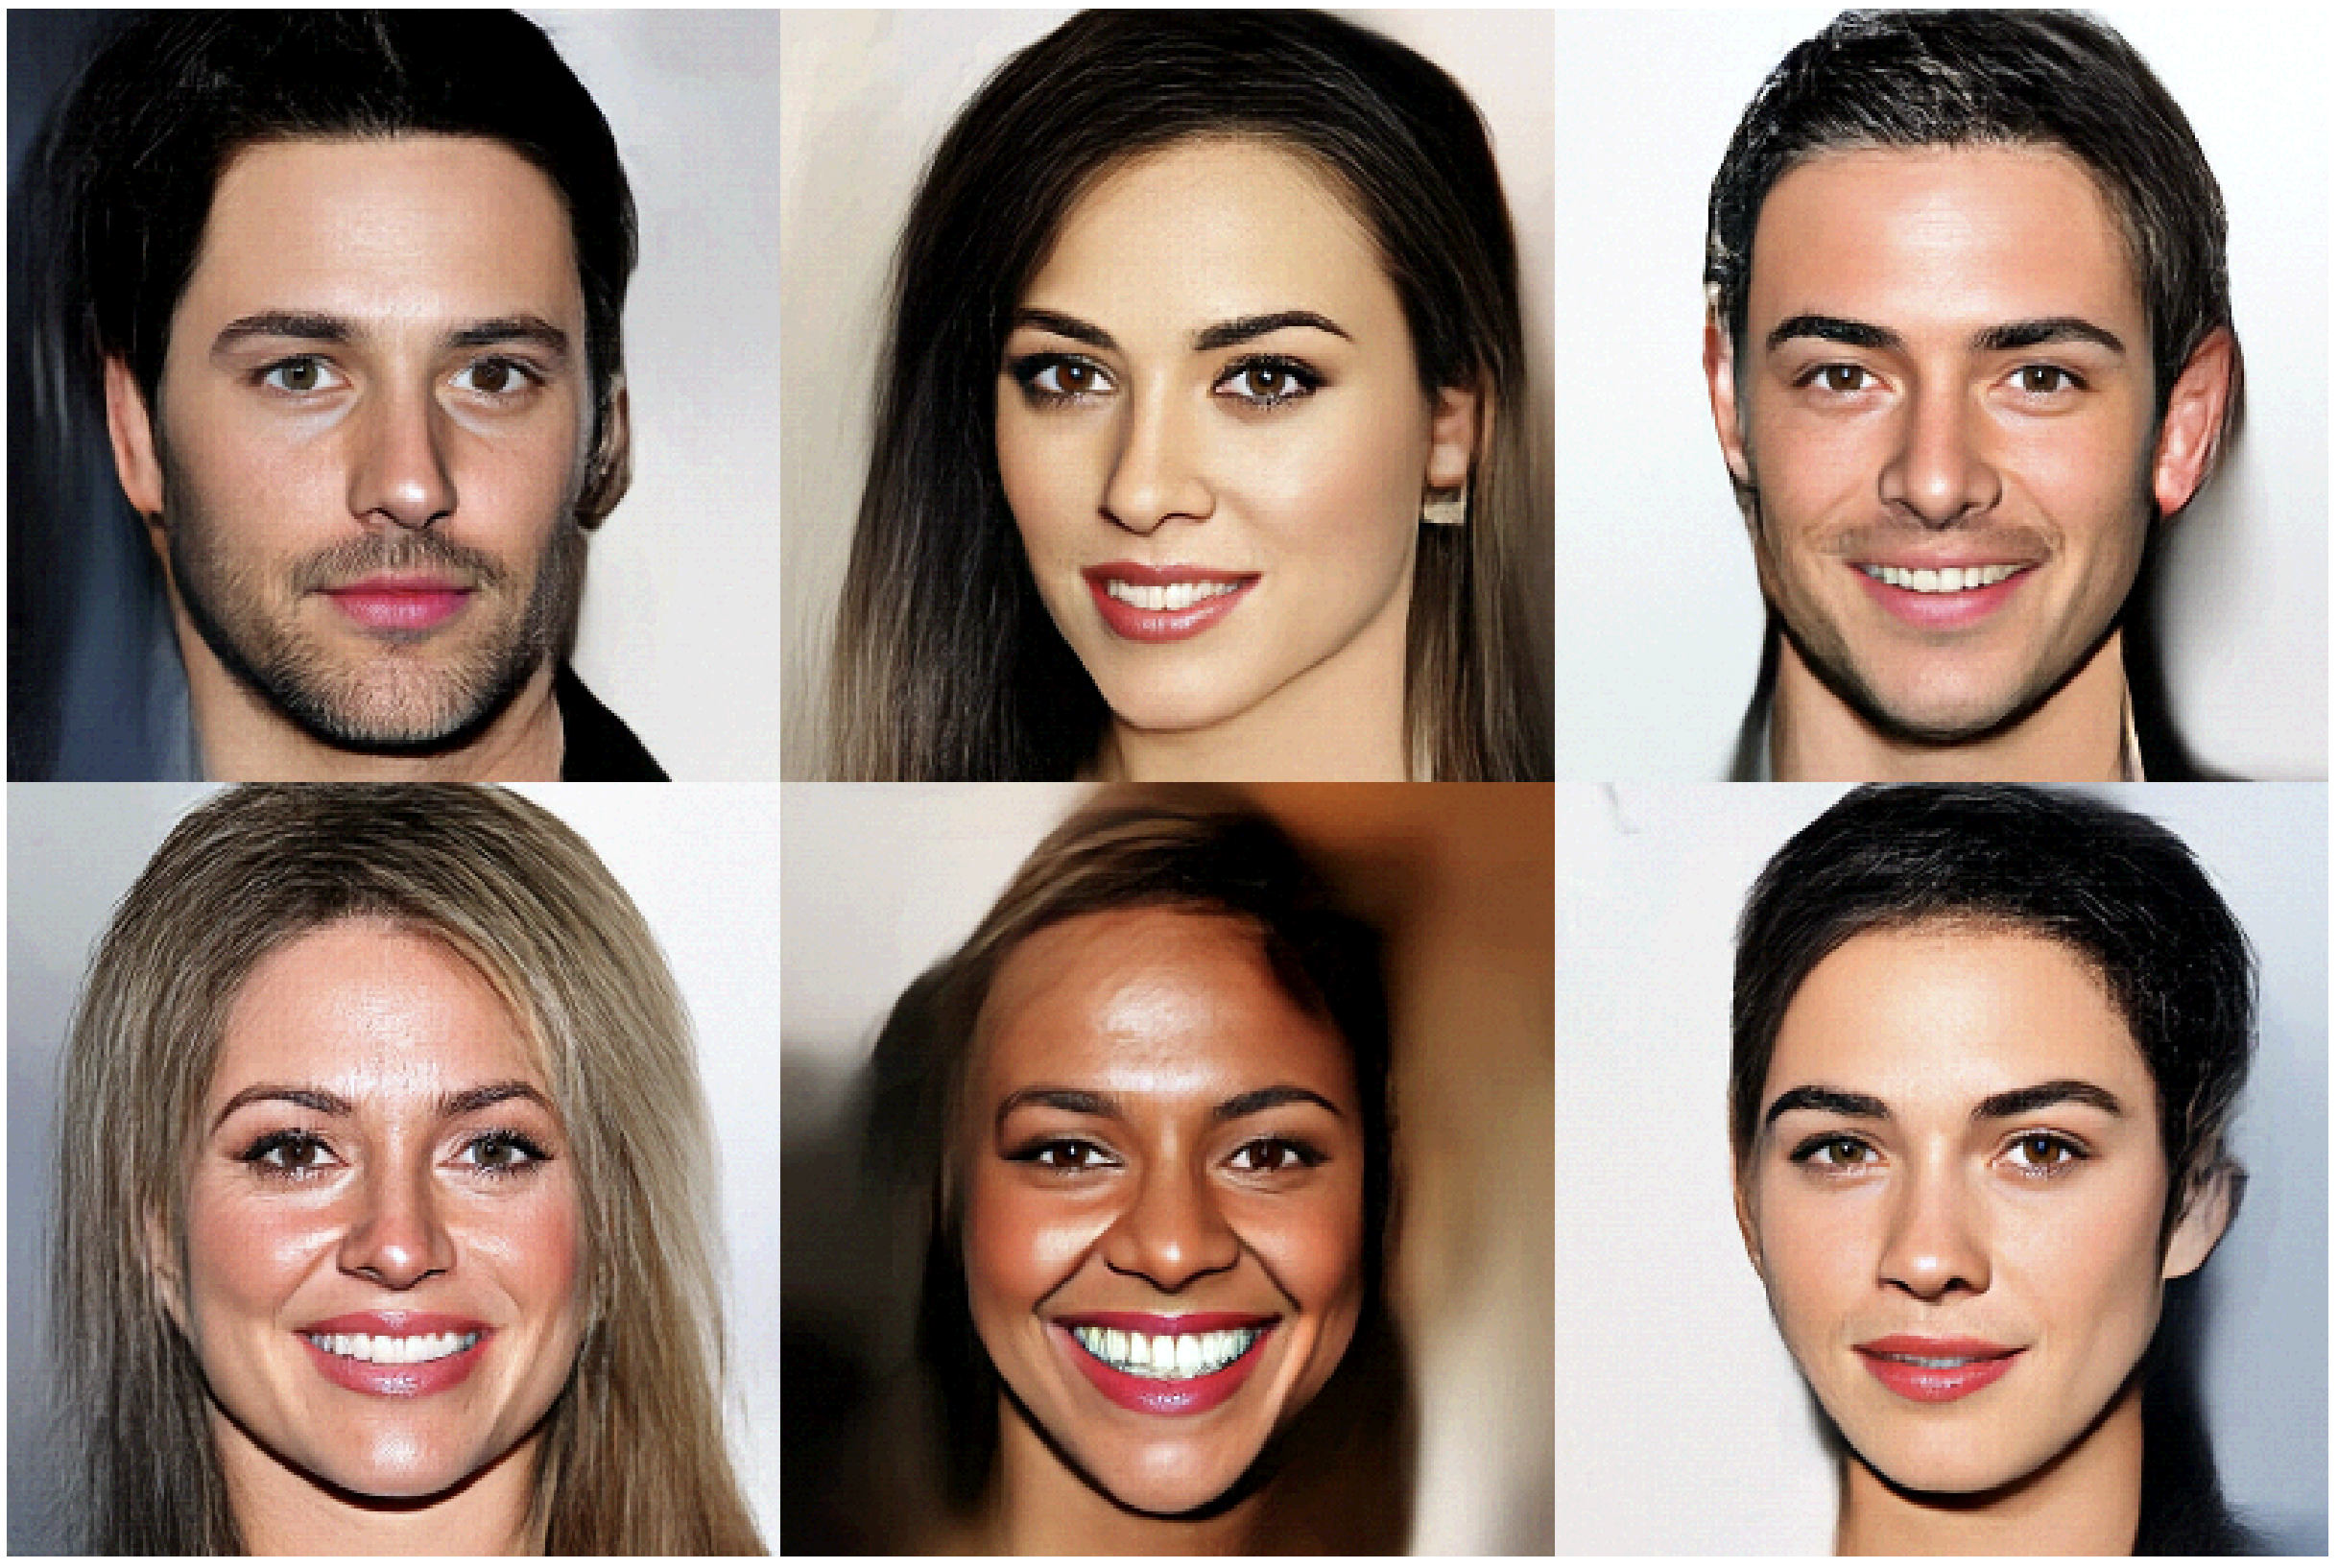
\includegraphics[width=\linewidth]{figs/glow_faces.png}
	\end{figure}
	\myfootnotewithlink{https://arxiv.org/abs/1807.03039}{Kingma D. P., Dhariwal P. Glow: Generative Flow with Invertible 1x1 Convolutions, 2018}
\end{frame}
%=======
\begin{frame}{Summary}
	\begin{itemize}
		\item AF/IAF is a special case of autoregressive flows.
		\vfill
		\item The RealNVP is an effective type of flow (special case of AR flows) that uses coupling layer.
	\end{itemize}
\end{frame}
%=======
\end{document} 